% !TEX encoding = UTF-8
% !TEX TS-program = pdflatex
% !TEX root = ../thesis.tex

%************************************************
\chapter{Hadronic Higgs Production}\label{chap:three}
%************************************************

\section{Motivation (better title needed!)}
Here I list various application for the Higgs production cross section and explain why precise predictions are so central. Maybe just put this in the chapter description?
\section{The Leading-Order Cross Section}
Having established, that the gluon-fusion Higgs production cross section is central for many phenomenological applications, we now want to perform the actual \acs{LO} calculation, which was first demonstrated by Georgi et al.\ in 1978~\cite{Georgi:1977gs}. The calculation not only serves as an instructive example on cross section calculation, and thereby allows us to put our experience from section~\ref{sec:2:cross_sections} to good use, but it already introduces many important concepts we can transfer to the \acs{NNLO} computation.

At LO, there are only two possible Feynman diagrams we can draw. They are depicted in Fig.~\ref{fig:4:LO}.
\begin{figure}[h]
\centering
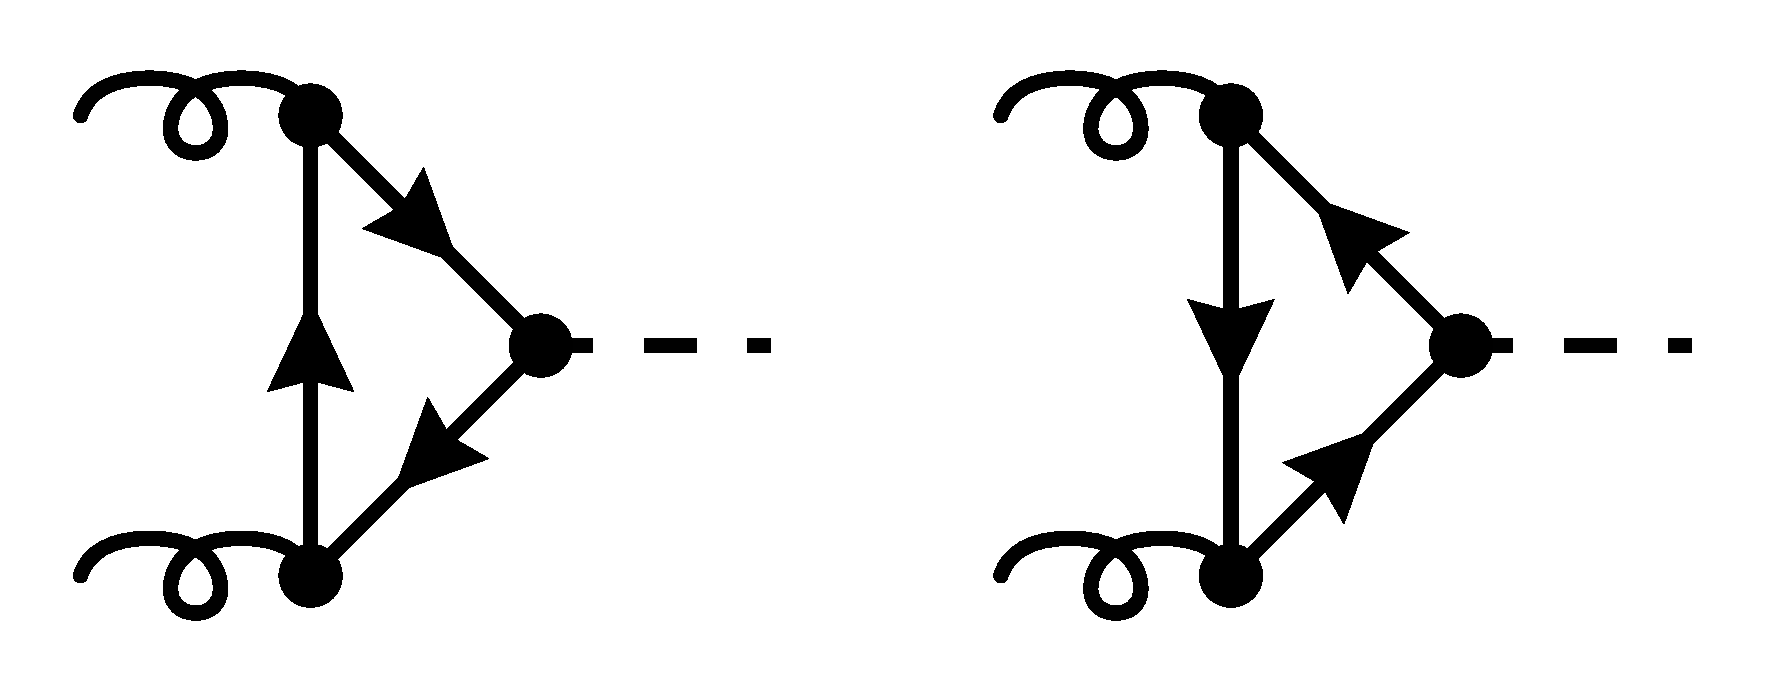
\includegraphics[scale=0.2]{Images/LO.pdf}
\caption{\acs{LO} Feynman diagrams for Higgs production in the gluon-fusion channel.}
\label{fig:4:LO}
\end{figure}
As we can see. Gluon-fusion is a loop induced process with two scales: the mass of the quark running in the loop $m_q$, and the Higgs mass $m_H$ which must simultaneously be the partonic center of mass energy. The initial state gluons carry on the on-shell momenta $p_1$ and $p_2$. Let us then define
\begin{equation}
i\mathcal{M} = i \mathcal{M}^{\mu\nu, ab} \varepsilon_\mu^a(p_1) \varepsilon_\nu^b(p_2).
\end{equation}
With the Feynman rules presented in appendix~\ref{app:1} we find
\begin{equation}
\begin{split}
&i \mathcal{M}^{\mu \nu, ab} = -\int \frac{\dd^4 k}{(2\pi)^4}\, \\
&\quad \times \text{Tr}\!\left[ \frac{-i m_q}{v} \delta_{ij} \frac{i(\slashed{k} + \slashed{p}_1 + \slashed{p}_2 + m_q)}{(k + p_1 + p_2)^2 - m_q^2} (ig \gamma^\nu T^a_{ik}) \frac{i (\slashed{k} + \slashed{p}_1 + m_q)}{(k + p_1)^2 - m_q^2} (i g \gamma^\mu T^b_{kj}) \frac{i (\slashed{k} + m_q)}{k^2 - m_q^2} \right] \\
&\quad + \lbrace p_1 \longleftrightarrow p_2,  \mu \longleftrightarrow \nu, a \longleftrightarrow b \rbrace ,
\label{eq:4:form_factor_amplitude}
\end{split}
\end{equation}
where the extra minus sign in front stems from the fermion trace.

Even without performing the explicit calculation can we already anticipate the general structure of the amplitude. Color wise, the amplitude must be proportional to $\delta^{ab}$, because it is the only symmetric rank-two tensor, which we require in order to satisfy \textit{Bose symmetry}. Similarly, $\mathcal{M}^{\mu\nu,ab}$ must also be a symmetric rank-two tensor in Minkowski space. The only building blocks we have available are $g^{\mu\nu}$, $(p_1^\mu p_2^\nu + p_2^\mu p_1^\nu)$, $p_1^\mu p_1^\nu$, and $p_2^\mu p_2^\nu$, but since all transverse parts drop out of the physical amplitude we are left with only $g^{\mu \nu}$ and $p_2^\mu p_1^\nu$. Lastly, we know that the amplitude must satisfy the \textit{Ward identity}, which allows us to restrict the tensor even further, such that we end up with
\begin{equation}
i \mathcal{M}^{\mu \nu, ab} = i\frac{\alphas}{\pi} \frac{1}{v} \delta^{ab} \left(p_2^\mu p_1^\nu - (p_1 \cdot p_2)g^{\mu\nu} \right) \mathcal{C}(m_H, m_q).
\label{eq:4:form_factor}
\end{equation}
Notice that we have only made use of very general properties of the amplitude. This is why the decomposition in Eq.~\eqref{eq:4:form_factor} will hold at every order of $\alphas$. The function $\mathcal{C}(m_H, m_q)$ is called the \textit{Higgs form factor}. It has mass dimension 2, \ie\ its functional dependence on $m_q$ and $m_H$ must be through a mass ratio
\begin{equation}
\mathcal{C} (m_H, m_q) = \mathcal{C}(z), \quad \text{with} \quad z \equiv \frac{m_H^2}{4 m_q^2}.
\end{equation}
The factor of $1/4$ was introduced, so that the \textit{normal threshold} is located at $z = 1$. Mathematically, this means that $z = 1$ is a solution of the \textit{Landau equations}, while physically, we can interpret the singularity as the point where we have enough energy to produce the quark pair on-shell. We can now project onto the form factor with
\begin{equation}
\mathcal{C}(z) = \frac{\pi v}{i \alphas} \frac{1}{N_c} \delta^{ab} \frac{1}{(p_1 \cdot p_2)^2 (d - 2)} \left(p_{2\,\mu} p_{1\,\nu} - (p_1 \cdot p_2) g_{\mu\nu} \right) i \mathcal{M}^{\mu \nu, ab}.
\end{equation}
If we now insert the \acs{LO} expression of Eq.~\eqref{eq:4:form_factor_amplitude} and perform some basic manipulations we find
\begin{equation}
\begin{split}
\mathcal{C}^{(0)} (z) = T_F \frac{1}{2 - 2 \epsilon} \frac{1}{z} \int \frac{\dd^d k}{i \pi^{d/2}} \,&\frac{1}{[k^2 - m_q^2 + i0^+][(k + p_1 + p_2)^2 - m_q^2 + i0^+]} \\
& \times \left( 2 \epsilon + \frac{m_H^2}{[(k + p_1)^2 - m_q^2 + i0^+]} \left(\frac{1}{z} + \epsilon - 1 \right) \right),
\end{split}
\end{equation}
which, after inserting integrals and expanding in $\epsilon$, finally reduces to
\begin{equation}
\mathcal{C}^{(0)}(z) = T_F \frac{1}{z} \bigg \lbrace 1 - \left(1 - \frac{1}{z} \right) \left[ \frac{1}{2} \ln\! \left( \frac{\sqrt{1 - 1/z} - 1}{\sqrt{1 - 1/z} + 1} \right) \right]^2 \bigg \rbrace.
\end{equation}


\section{The Heavy-Top Limit}
Here I explain the heavy-top limit.
\section{Higher-Order Corrections}
Here I outline how to perform higher order corrections.
\section{Theory Status}
Here I describe what is already known about the gluon-gluon fusion channel. I explain the theory uncertainties.

